\documentclass[11pt,a4paper]{article}
\usepackage{../common/polycopie_style}

\begin{document}

\makepolycopieheader{Choix Méthodologique, Puissance \& Bonnes Pratiques}{Arbre de Décision, Éthique Expérimentale \& Standards de Publication}{CHAPITRE 7}

\section{Introduction : La Crise de la Reproductibilité en Biologie}

Ces dernières années, plus de 70\% des chercheurs en biomédecine ont rapporté avoir échoué à reproduire des résultats publiés dans des revues prestigieuses. Les causes majeures de cette crise ne sont pas des fraudes délibérées, mais des \textbf{défauts méthodologiques fondamentaux} :
\begin{itemize}[leftmargin=*, label=\faAngleRight]
  \item Échantillons animaux dramatiquement sous-dimensionnés ($n = 3$ souris par lot).
  \item Multiplication des tests statistiques sans correction du risque global d'erreur.
  \item Arrêt précoce des expériences dès qu'un $p < 0.05$ est obtenu par hasard.
  \item Utilisation de représentations graphiques trompeuses masquant la réalité des données.
\end{itemize}

Ce chapitre fournit au futur biochimiste la boîte à outils méthodologique pour \textbf{concevoir des expériences valides, éthiques et reproductibles}.

\section{L'Arbre de Décision Statistique du Biologiste}

Face à un jeu de données expérimental, le choix du test statistique obéit à un algorithme décisionnel strict :

\begin{figurebox}{Arbre Décisionnel des Tests Statistiques en Biologie}
\begin{center}
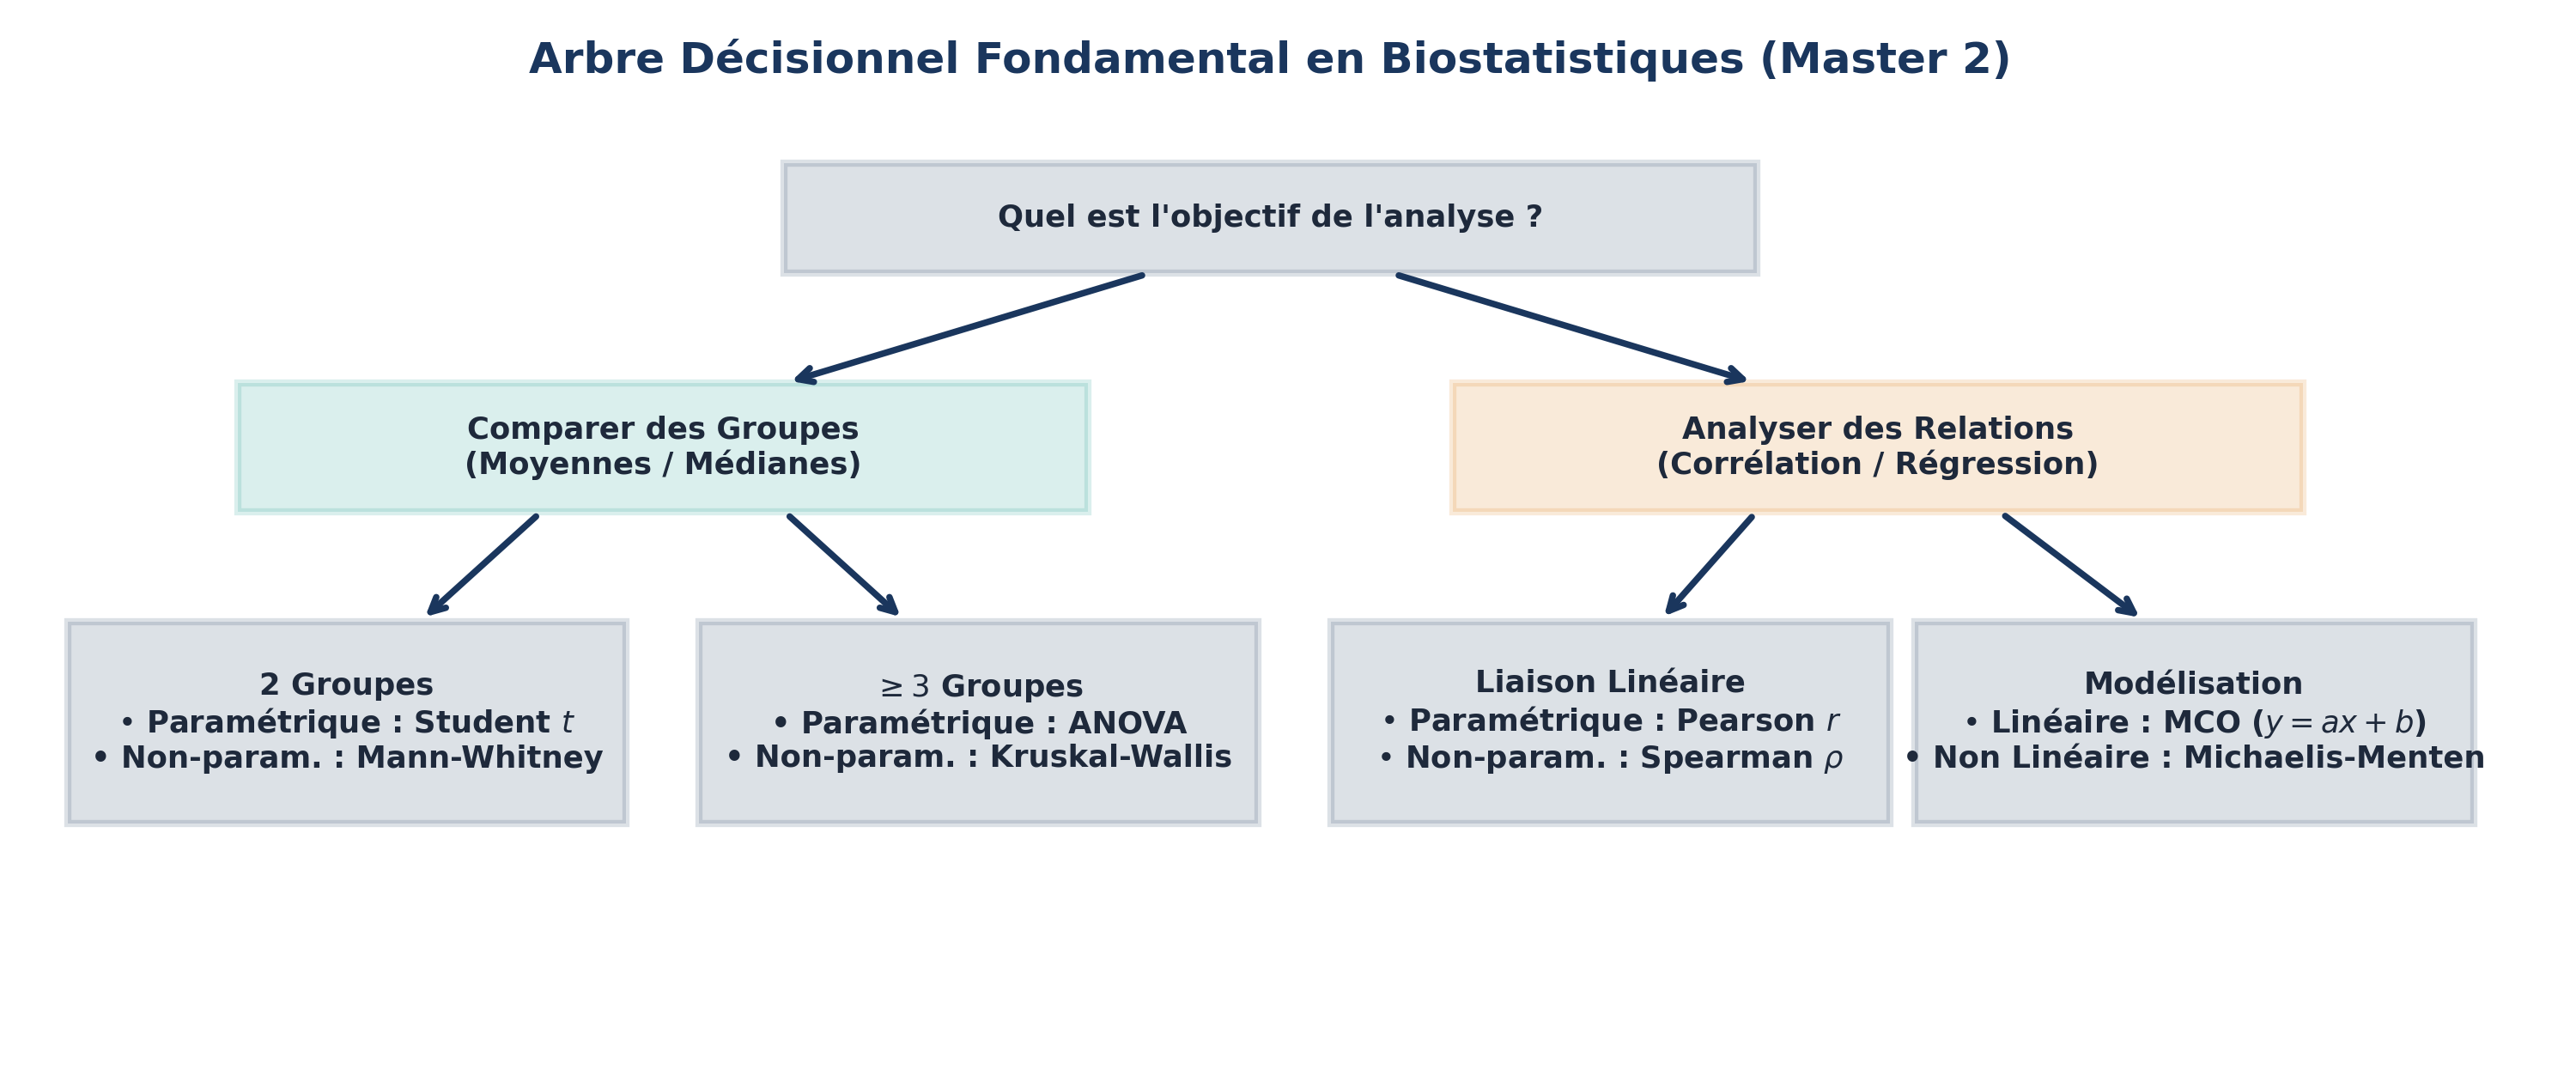
\includegraphics[width=0.86\linewidth]{../../sources/figures/fig00_decision_tree_tests.png}
\end{center}
\textbf{Cheminement méthodologique pour sélectionner le bon test :}
\begin{itemize}[leftmargin=*, label=\faAngleRight]
  \item \textbf{Type de variable :} Déterminer si la réponse est quantitative continue (absorbance, concentration, poids) ou qualitative discrète (survie, présence/absence).
  \item \textbf{Vérification des postulats :} Tester la normalité (Shapiro-Wilk) et l'égalité des variances (Levene/Bartlett). Si $p < 0.05$ ou effectifs très réduits ($n < 6$), basculer impérativement vers les tests non paramétriques (Wilcoxon, Mann-Whitney, Kruskal-Wallis).
  \item \textbf{Structure expérimentale :} Identifier si les mesures sont indépendantes (lots séparés) ou appariées/répétées (même animal suivi dans le temps).
\end{itemize}
\end{figurebox}

\begin{center}
\resizebox{\linewidth}{!}{%
\begin{tabular}{llll}
\toprule
\textbf{Question Biologique} & \textbf{Conditions Normales (Paramétrique)} & \textbf{Non-Normalité / Petits Échantillons} \\
\midrule
Comparer 1 groupe à une valeur théorique & Test $t$ de Student pour échantillon unique & Test de Wilcoxon signé \\
Comparer 2 groupes indépendants (Témoin vs Traité) & Test $t$ de Student pour échantillons indépendants & Test $U$ de Mann-Whitney \\
Comparer 2 mesures appariées (Avant vs Après) & Test $t$ de Student pour mesures appariées & Test de Wilcoxon pour séries appariées \\
Comparer $\ge 3$ groupes à 1 facteur & ANOVA à 1 facteur (One-Way) & Test de Kruskal-Wallis \\
Comparer des mesures répétées ($\ge 3$ temps) & ANOVA pour mesures répétées & Test de Friedman \\
Tester 2 facteurs croisés et leur interaction & ANOVA à 2 facteurs croisés (Two-Way) & Modèles Linéaires Mixtes / Rangs alignés \\
Facteur emboîté (lots, cuves, sous-échantillons) & ANOVA hiérarchisée (Nested ANOVA) & Modèles Mixtes Hiérarchiques \\
Liaison entre deux variables continues & Régression Linéaire / Corrélation Pearson & Corrélation des rangs de Spearman \\
\bottomrule
\end{tabular}%
}
\end{center}

\section{Puissance Statistique ($1-\beta$) \& Calcul d'Effectif ($N$)}

Un test statistique est soumis à deux types d'erreurs :
\begin{itemize}[leftmargin=*, label=\faCheck]
  \item \textbf{Erreur de Type I ($\alpha$, Faux Positif) :} Conclure à un effet biologique alors qu'il n'y en a aucun (fixé conventionnellement à $\alpha = 0.05$).
  \item \textbf{Erreur de Type II ($\beta$, Faux Négatif) :} Manquer un effet biologique réel par manque de sensibilité de l'expérience.
  \item \textbf{Puissance Statistique ($1 - \beta$) :} La probabilité de détecter un effet réel existant (standard international : $1 - \beta \ge 80\%$).
\end{itemize}

\begin{conceptbox}{La Taille d'Effet Standardisée ($d$ de Cohen)}
Pour dimensionner une étude, on calcule la taille d'effet biologique attendue :
\begin{equation*}
  d = \frac{|\mu_1 - \mu_2|}{\sigma}
\end{equation*}
L'effectif nécessaire par groupe pour $\alpha = 0.05$ et une puissance de $80\%$ s'obtient par la formule de Lehr :
\begin{equation*}
  n = \frac{2 \cdot (Z_{\alpha/2} + Z_\beta)^2}{d^2} \approx \frac{2 \cdot (1.960 + 0.842)^2}{d^2} \approx \frac{15.7}{d^2}
\end{equation*}
\end{conceptbox}

\begin{figurebox}{Courbes de Puissance Statistique ($1 - \beta$) vs Taille d'Échantillon ($N$)}
\begin{center}
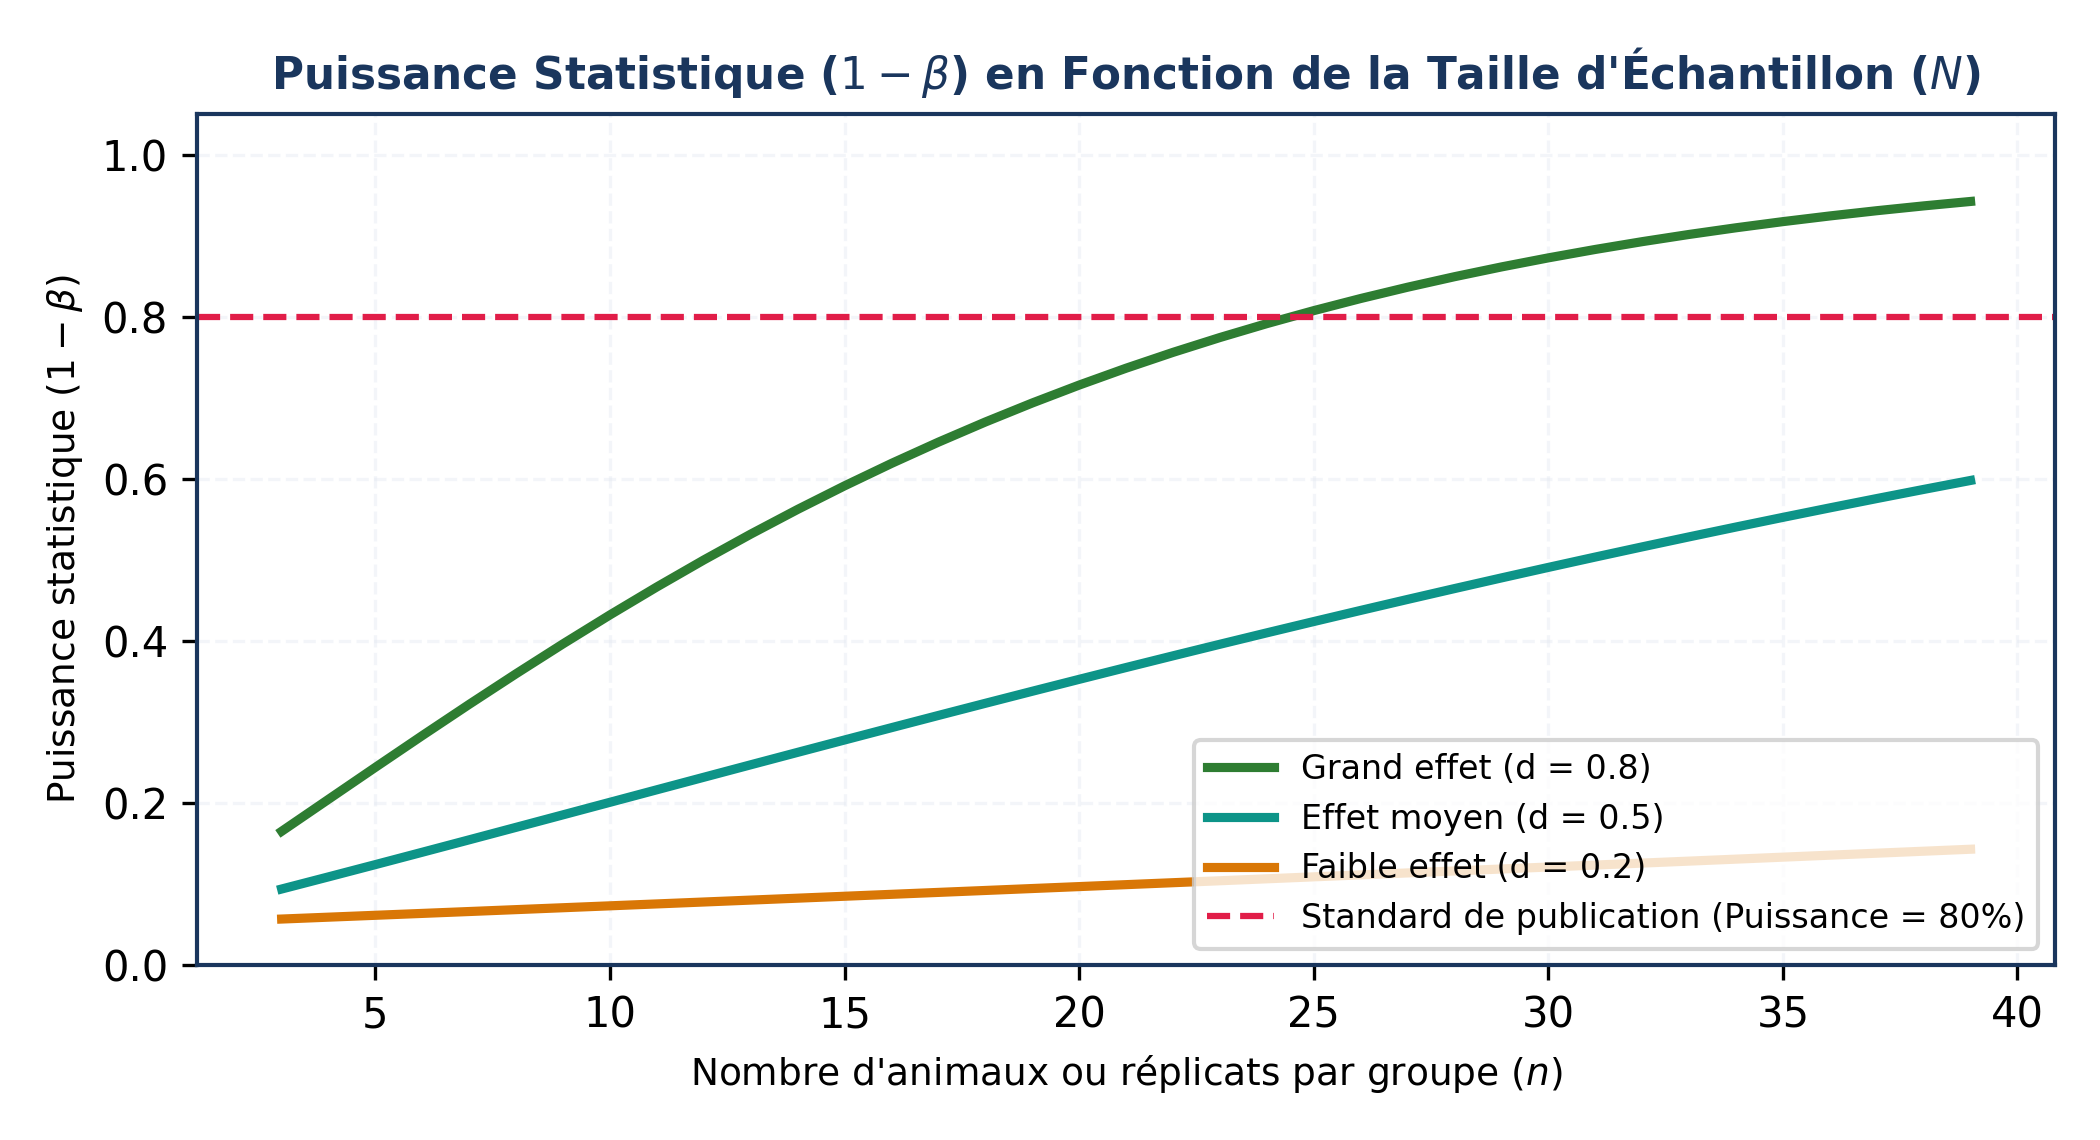
\includegraphics[width=0.86\linewidth]{../../sources/figures/fig07_power_sample_size_curve.png}
\end{center}
\textbf{Analyse des profils de puissance et du seuil cible de 80\% :}
\begin{itemize}[leftmargin=*, label=\faAngleRight]
  \item \textbf{Impact de la taille d'effet ($d$) :} Pour un effet modeste ($d = 0.2$), même $N = 50$ sujets ne suffit pas à atteindre 80\% de puissance. Pour un effet majeur ($d = 0.8$), $N = 25$ suffit amplement.
  \item \textbf{Danger des petits effectifs ($N \le 5$) :} Quelle que soit la puissance théorique, travailler avec des effectifs minuscules condamne l'étude à un risque massif de faux négatif ($\beta > 70\%$).
\end{itemize}
\end{figurebox}

\begin{warnbox}{Le Piège des Petits Échantillons \& la « Malédiction du Vainqueur »}
Avec $n = 3$ souris par lot, la puissance statistique est souvent inférieure à $20\%$. Dans ce régime de sous-puissance :
\begin{enumerate}
  \item L'expérience a 4 chances sur 5 d'échouer à détecter une molécule réellement active.
  \item Les rares études qui franchissent le seuil $p < 0.05$ par pure fluctuation aléatoire surestiment massivement la taille de l'effet biologique (\textit{Winner's Curse}).
\end{enumerate}
\end{warnbox}

\section{Comparaisons Multiples \& Contrôle du Faux Taux de Découverte (FDR)}

Lorsqu'un chercheur teste simultanément $m = 20$ gènes ou métabolites sans correction :
\begin{equation*}
  \alpha_{\text{global}} = 1 - (1 - 0.05)^{20} = 1 - (0.95)^{20} \approx 1 - 0.358 = \mathbf{64.2\%}
\end{equation*}
Il y a plus de 64\% de chances de déclarer à tort au moins une variable significative par pur hasard !

\subsection{L'Algorithme Pas-à-Pas de Benjamini-Hochberg (FDR)}
\begin{enumerate}[leftmargin=*, label=\faCalculator\ \textbf{\arabic*.}]
  \item Classer les $m$ valeurs $p$ brutes par ordre croissant : $p_{(1)} \le p_{(2)} \le \dots \le p_{(m)}$.
  \item Pour chaque rang $i \in \{1, \dots, m\}$, calculer le seuil critique proportionnel : $q_i = \frac{i}{m} \times Q$ (où $Q$ est le taux de fausses découvertes toléré, souvent $Q = 0.05$).
  \item Identifier le plus grand rang $k$ tel que $p_{(k)} \le \frac{k}{m} \times Q$.
  \item Rejeter toutes les hypothèses nulles pour les rangs $1, 2, \dots, k$ (déclarées biologiquement significatives).
\end{enumerate}

\section{Transparence Graphique : L'Abandon des Barplots « Dynamite »}

Pendant des décennies, la biologie a représenté les données quantitatives sous forme d'histogrammes en barres pleines surmontées d'un écart-type.

\begin{figurebox}{Transparence Graphique : Barplot Dynamite vs Boxplot de Tukey + Jitter}
\begin{center}
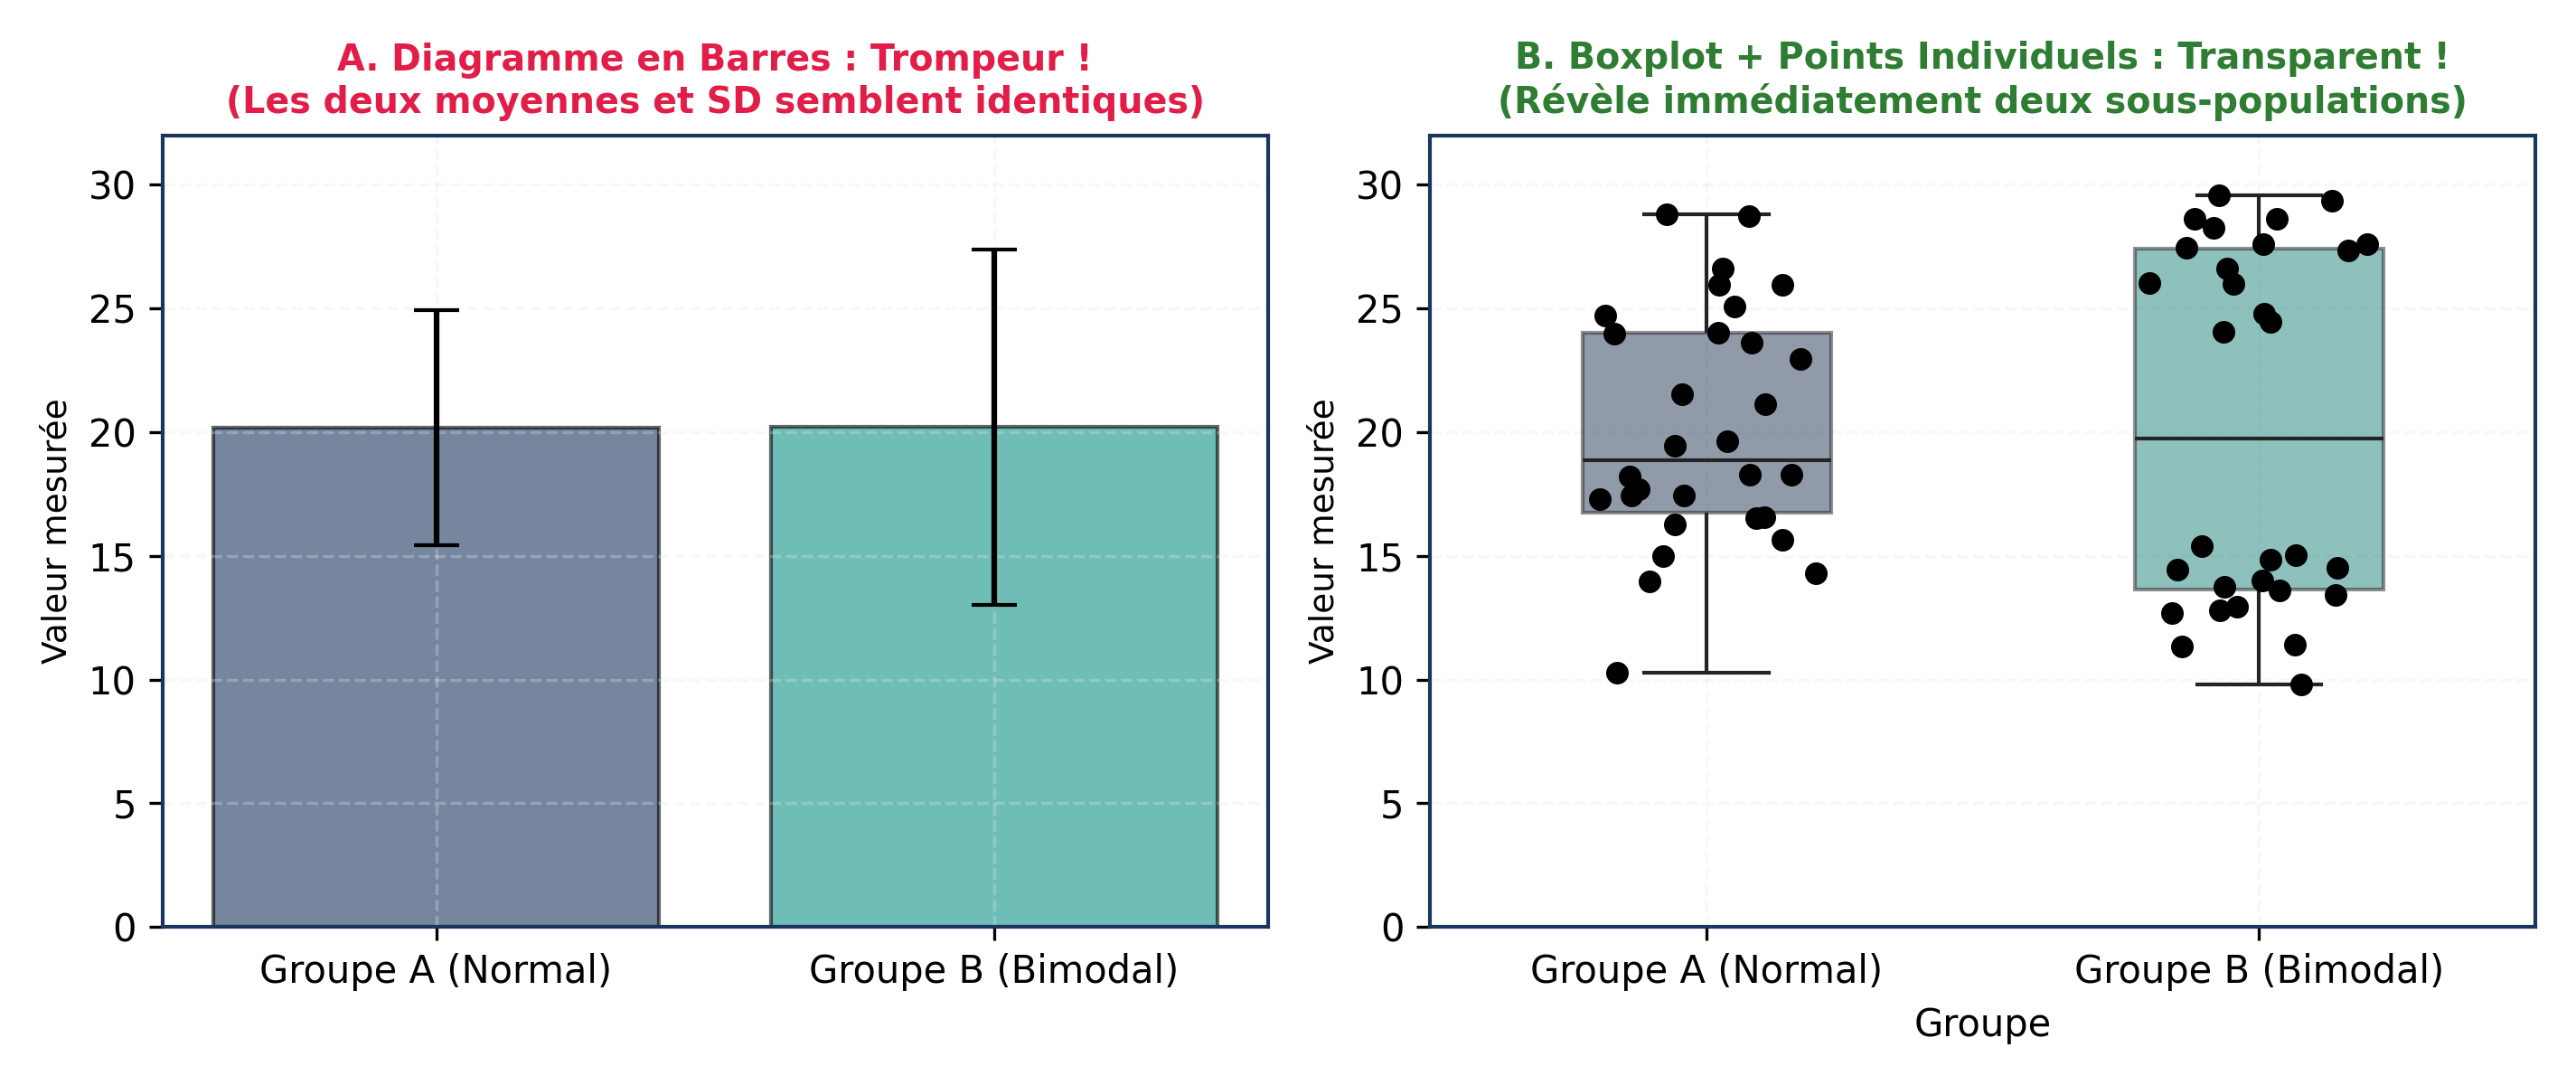
\includegraphics[width=0.86\linewidth]{../../sources/figures/fig07_barplot_vs_boxplot_transparency.png}
\end{center}
\textbf{Comparaison sans appel entre les deux représentations :}
\begin{itemize}[leftmargin=*, label=\faAngleRight]
  \item \textbf{Barplot « Dynamite » (Gauche) :} Donne une illusion trompeuse d'homogénéité. Deux populations aux distributions diamétralement opposées (l'une normale, l'autre bimodale avec deux sous-groupes cliniques) produisent exactement le même barplot !
  \item \textbf{Boxplot + Jitter Plot (Droite) :} Révèle instantanément la véritable structure des données : la médiane, l'écart interquartile, les valeurs extrêmes et la présence de deux sous-populations distinctes de patients répondeurs.
\end{itemize}
\end{figurebox}

\begin{takeawaybox}{Règle de Publication : Le Boxplot Enrichi des Points Individuels}
Les revues majeures (\textit{Nature, Cell, PLOS}) interdisent formellement les barplots pour les petits effectifs ($n < 30$) car une barre pleine :
\begin{enumerate}
  \item Masque totalement la bimodalité (deux sous-populations non répondeuses / hyper-répondeuses).
  \item Dissimule les valeurs aberrantes (outliers) et l'asymétrie de la distribution.
\end{enumerate}
\textbf{Standard d'excellence :} Toujours tracer un \textbf{Boxplot de Tukey} (médiane, quartiles $Q_1, Q_3$, moustaches) superposé à \textbf{la totalité des points expérimentaux bruts} (\textit{jitter plot}).
\end{takeawaybox}

\section{Exercices d'Application \& Solutions}

\begin{exercicebox}{Exercice 1 : Taille d'Effet ($d$ de Cohen) \& Dimensionnement Expérimental}
Une équipe évalue l'effet hépatoprotecteur d'une molécule sur le MDA hépatique ($\mu\text{mol/g}$) chez le rat :
\begin{itemize}
  \item Taux basal chez les témoins : $\mu_1 = 8.5\,\mu\text{mol/g}$, écart-type $s = 2.0\,\mu\text{mol/g}$.
  \item Amélioration minimale biologiquement pertinente : $\mu_2 = 6.5\,\mu\text{mol/g}$ ($\Delta = 2.0\,\mu\text{mol/g}$).
  \item Paramètres requis : $\alpha = 0.05$ ($Z_{\alpha/2} = 1.960$), puissance souhaitée $1 - \beta = 80\%$ ($Z_\beta = 0.842$).
\end{itemize}
\begin{enumerate}[label=\textbf{\alph*.}]
  \item Calculez la taille d'effet standardisée ($d$ de Cohen).
  \item Déterminez le nombre d'animaux nécessaire par groupe ($n$).
  \item Si l'expérimentateur n'utilise que $n = 3$ rats par groupe, que devient la puissance statistique ?
  \item Expliquez les conséquences éthiques et scientifiques de travailler avec un effectif sous-dimensionné.
\end{enumerate}
\end{exercicebox}

\begin{solutionbox}{Solution : Exercice 1}
\begin{enumerate}[label=\textbf{\alph*.}]
  \item \textbf{Taille d'effet de Cohen ($d$) :}
  \begin{equation*}
    d = \frac{|\mu_1 - \mu_2|}{s} = \frac{|8.5 - 6.5|}{2.0} = \frac{2.0}{2.0} = \mathbf{1.00} \quad (\text{Effet biologique fort})
  \end{equation*}
  \item \textbf{Calcul du nombre d'animaux ($n$) :}
  \begin{align*}
    n &= \frac{2 \cdot (Z_{\alpha/2} + Z_\beta)^2}{d^2} = \frac{2 \cdot (1.960 + 0.842)^2}{1.00^2} \\
    &= 2 \times (2.802)^2 = 2 \times 7.851 = \mathbf{15.7} \implies \mathbf{n = 16 \text{ rats/lot}}
  \end{align*}
  Il faut donc $16$ animaux par groupe (soit $N = 32$ rats au total) pour garantir 80\% de chances de détecter cet effet au seuil $\alpha = 5\%$.
  \item \textbf{Conséquence avec $n = 3$ rats :}
  Avec $n = 3$, $Z_\beta = d \sqrt{n/2} - Z_{\alpha/2} = 1.0 \times \sqrt{1.5} - 1.960 = 1.225 - 1.960 = -0.735$.
  La puissance correspondante est de seulement $\mathbf{23\%}$ (plus de 3 chances sur 4 d'échouer à observer la significativité !).
  \item \textbf{Conséquences scientifiques et éthiques :}
  \begin{itemize}
    \item \textbf{Gaspillage éthique (règle des 3R) :} Sacrifier 6 animaux pour une étude vouée à l'inconclusivité statistique est contraire à l'éthique animale.
    \item \textbf{Non-reproductibilité :} Si par hasard le test ressort significatif ($p < 0.05$), c'est par une fluctuation d'échantillonnage extrême qui ne sera jamais reproduite par d'autres laboratoires.
  \end{itemize}
\end{enumerate}
\end{solutionbox}

\begin{exercicebox}{Exercice 2 : Comparaisons Multiples \& Procédure FDR de Benjamini-Hochberg}
Une étude métabolomique compare $m = 10$ acides aminés plasmatiques entre témoins et patients diabétiques. Les 10 tests $t$ fournissent les $p$-valeurs brutes suivantes ordonnées :
\begin{center}
\small
\begin{tabular}{ccccccccccc}
\toprule
\textbf{Rang ($i$)} & 1 & 2 & 3 & 4 & 5 & 6 & 7 & 8 & 9 & 10 \\
\midrule
\textbf{$p$-valeur brute} & 0.002 & 0.008 & 0.012 & 0.021 & 0.039 & 0.055 & 0.082 & 0.120 & 0.250 & 0.640 \\
\bottomrule
\end{tabular}
\end{center}
\begin{enumerate}[label=\textbf{\alph*.}]
  \item Sans correction, combien de métabolites paraissent « statistiquement significatifs » au seuil classique $\alpha = 0.05$ ?
  \item Appliquez la correction conservative de Bonferroni au seuil $\alpha = 0.05$ ($\alpha' = 0.05 / 10 = 0.005$). Quels métabolites restent significatifs ?
  \item Appliquez la procédure FDR de Benjamini-Hochberg au taux de faux positifs $Q = 0.05$ en comparant chaque $p$-valeur au seuil critique glissant :
  \begin{equation*}
    p_{(i)} \le \frac{i}{m} \cdot Q = \frac{i}{10} \times 0.05
  \end{equation*}
  \item Comparez le résultat des deux méthodes et concluez sur le plan biologique.
\end{enumerate}
\end{exercicebox}

\begin{solutionbox}{Solution : Exercice 2}
\begin{enumerate}[label=\textbf{\alph*.}]
  \item \textbf{Sans correction ($\alpha = 0.05$) :}
  Toutes les $p$-valeurs $< 0.05$ sont retenues : rangs 1, 2, 3, 4 et 5 $\implies$ \textbf{5 métabolites} déclarés significatifs. Mais le risque d'au moins un faux positif parmi eux est de $1 - (0.95)^{10} = \mathbf{40.1\%}$ !
  \item \textbf{Correction de Bonferroni ($\alpha' = 0.005$) :}
  Seule la $p$-valeur du rang 1 ($p = 0.002 \le 0.005$) franchit le seuil.
  $\implies$ \textbf{1 seul métabolite} retenu (les métabolites 2, 3, 4, 5 sont perdus par excès de sévérité).
  \item \textbf{Procédure FDR de Benjamini-Hochberg ($Q = 0.05$) :}
  Calculons le seuil critique pour chaque rang $i$ :
  \begin{itemize}
    \item Rang 1 : $p_{(1)} = 0.002 \le \frac{1}{10} \times 0.05 = \mathbf{0.005}$ \quad (Vrai)
    \item Rang 2 : $p_{(2)} = 0.008 \le \frac{2}{10} \times 0.05 = \mathbf{0.010}$ \quad (Vrai)
    \item Rang 3 : $p_{(3)} = 0.012 \le \frac{3}{10} \times 0.05 = \mathbf{0.015}$ \quad (Vrai)
    \item Rang 4 : $p_{(4)} = 0.021 \le \frac{4}{10} \times 0.05 = \mathbf{0.020}$ \quad (\textbf{Faux} : $0.021 > 0.020$)
  \end{itemize}
  Le plus grand rang $k$ tel que $p_{(k)} \le \frac{k}{m} Q$ est \textbf{$k = 3$} ($p_{(3)} = 0.012 \le 0.015$).
  On retient donc tous les métabolites de rang $1 \le i \le 3$ : \textbf{les métabolites 1, 2 et 3}.
  \item \textbf{Synthèse biologique :}
  La méthode FDR permet de repêcher les métabolites 2 et 3 (rejetés à tort par Bonferroni), tout en éliminant les métabolites 4 et 5 qui n'étaient que du bruit d'échantillonnage. Elle offre le parfait équilibre entre découverte biologique et rigueur statistique.
\end{enumerate}
\end{solutionbox}

\section*{Formulaire Récapitulatif : Les Bonnes Pratiques de Laboratoire}
\begin{center}
\resizebox{\linewidth}{!}{%
\begin{tabular}{lll}
\toprule
\textbf{Notion Clé} & \textbf{Formule / Référence} & \textbf{Conséquence Pratique en Recherche} \\
\midrule
Taille d'effet standardisée & $d = |\mu_1 - \mu_2| / \sigma$ & Quantifie l'importance biologique réelle indépendamment de $N$ \\
Formule d'effectif (Lehr) & $n \approx 15.7 / d^2$ & Calcule le nombre minimal d'animaux pour une puissance de 80\% \\
Risque d'erreur global & $\alpha_{\text{global}} = 1 - (1 - \alpha)^m$ & Montre l'inflation rapide des faux positifs lors de tests multiples \\
Seuil de Bonferroni & $\alpha' = \alpha / m$ & Contrôle strict du Family-Wise Error Rate (très conservateur) \\
Benjamini-Hochberg FDR & $p_{(i)} \le \frac{i}{m} Q$ & Standard omique : contrôle le taux de fausses découvertes \\
Graphiques de données & Boxplot + Jitter plot & Remplace les barplots pour révéler la distribution intégrale \\
\bottomrule
\end{tabular}%
}
\end{center}

\end{document}
